\documentclass[a4paper,12pt]{book}
\usepackage[utf8]{inputenc}
\usepackage{graphicx}
\usepackage{fixltx2e}
\graphicspath{ {images/} }
\title{Computing Practical Project}
\author{Oscar Daniel}
\date{Febuary 2015 }
\begin{document}



\maketitle
\tableofcontents

\chapter{Analysis}

\section{Background and Definition of Problem}
\begin{flushleft}
At Queen Elizabeth Grammar School, pupils in year 13 are taught several calculations for their science subjects. They are tested on these every month or so, after the unit has been taught and students are assumed to understand the topics. Students are set questions during teaching time, however these results are not recorded and sometimes a struggling student may slip under a teacher’s radar.
\\Calculations follow:\\
\textbf{Rate of reaction equations}\\
A set of reaction equations used to deduce the rate of a reaction, the concentrations of reactants, their orders and the rate constant: k. \\
A reaction of reactants A + B 

\emph{An example question.}	\\
\textbf{Standard deviation}\\
 A statistical value that is used ceaselessly in biology.\\
         You and your friends have just measured the heights of your dogs (in millimetres):

         The heights (at the shoulders) are: 600mm, 470mm, 170mm, 430mm and 300mm.
	Find the standard deviation\\
Find out the Mean, the Variance, and the Standard Deviation.\\
Your first step is to find the Mean:
The mean (average) height is 394 mm\\
Now we calculate each dog's difference from the Mean. To calculate the Variance, take each difference, square it, and then average the result:

So, the Variance is 21,704.\\
And the Standard Deviation is just the square root of Variance, so:
Standard Deviation: sqrt of  21,704 = 147.32  = 147 (to the nearest mm)\\


         \emph{ An Example Question}\\
\textbf{Ideal Gas Equation}\\  A calculation that is used in both chemistry and physics A level.\\
The ideal gas equation is PV = nRT. P is pressure in Pa, V is volume in cubic metres, n is number of moles and T is temperature in degrees Kelvin. R is the ideal gas constant which is measured as 8.314 Joules per Kelvin per Mole.\\
STP = 273K and 100kPa\\
Problem 1: Determine the volume of occupied by 2.34 grams of carbon dioxide gas at STP.\\
Our first job is to rearrange the equation to find V: V = nRT/P\\
Then find moles of CO\textsubscript{2}: 2.34/44 =  0.0532\\
Then apply these to the equation.\\
$ (0.0532*8.314*273)/100,000 = 0.0012074921  m^3 $\\
Problem 2: A sample of argon gas at STP occupies 56.2 litres. Determine the number of moles of argon and the mass in the sample.\\
Rearrange to find n: n=PV/RT\\
56.2  litres = 0.0000562 $ m^3 $\\
(100,000*0.0000562)/(8.314*273) = 0.00247607416 moles. $ Ar = 18g/Mole $\\
$ 18*0.00248 = 0.0446g $\\
\emph{An Example Question}\\
Hardy – Weinberg Equation: A statistical test that is used to estimate the proportions of different genotypes in a population.\\
1. If 98 out of 200 individuals in a population express the recessive phenotype, what percent of the population would you predict would be heterozygotes?
(a) I have given you information on the frequency of the homozygous recessive (or q2). So start by determining q2 and then solving for q.  $ 98/200 =  q^2 = 0.49 $
sqrt 0.49 = 0.7 = q\\
(b) Now that you have q, you can solve for p. Remember there are only two alleles in the population, so if you add the frequency of the two alleles, you have accounted for all possibilities and it must equal 1. So p + q = 1. p = 1-q = 0.3\\
(c) Now what is the formula for heterozygotes? Think back to the Hardy-Weinberg equation -- it is dealing with the genotypes of individuals in the population.
$ 2pq = 2*0.3*0.7 = 0.42 $\\
(d) Now that you have figured out the % of heterozygotes, can you figure out the % of homozygous dominant? Does the % of homozygous dominant, heterozygotes and homozygous recessive individuals add up to 100%? If not, you have made an error. Those are the only three genotypes possible with only two alleles and a simple dominant and recessive relationship.
$ 1-(0.49 + 0.42) = p^2 = 0.09 or 0.3^2 $
An Example Question
\end{flushleft}


\section{Users and the current system}

Mr Fascione is the head of Science at QEGS.  He focusses on student grades and student support alongside being a teacher.\\
Currently the only way for pupils’ scores from homework to be tracked is by them being entered manually into a spreadsheet after being recorded on paper. There is also no way for pupils to have their problems solved, or explained step by step, other than referring to a text book, which is not interactive. Student feedback is also only monitored for tests, with this system every piece of homework could be used for student support.
Pupils can only access a few problems that have been devised by teachers or examiners. These can also be hard for students to grasp, so a program which goes through these at the students’ personal pace would be of great use. Teachers also have no digitally stored questions that can be easily sent to students, they must hand out photocopies and these are always being lost. A computer system would allow work to be set easily, without risk of students losing their things, as well as teachers not losing score sheets.
From my feedback and interviews from my end users I have been able to select the appropriate calculations for the computer package to use, and also have a framework to try and emulate, to best please my end user.\\


\section{Feedback Reports}
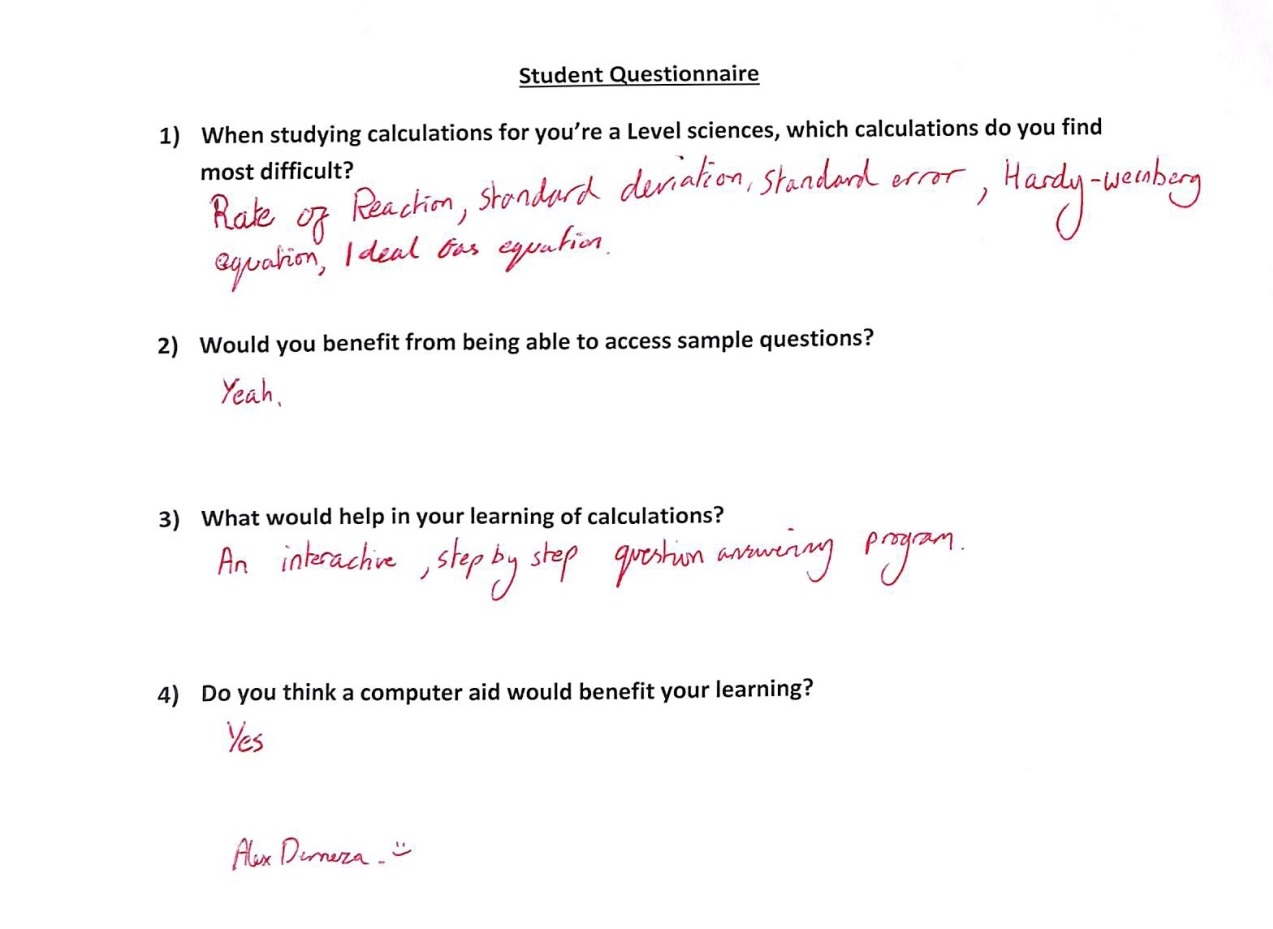
\includegraphics{StudentQuestionnaire}
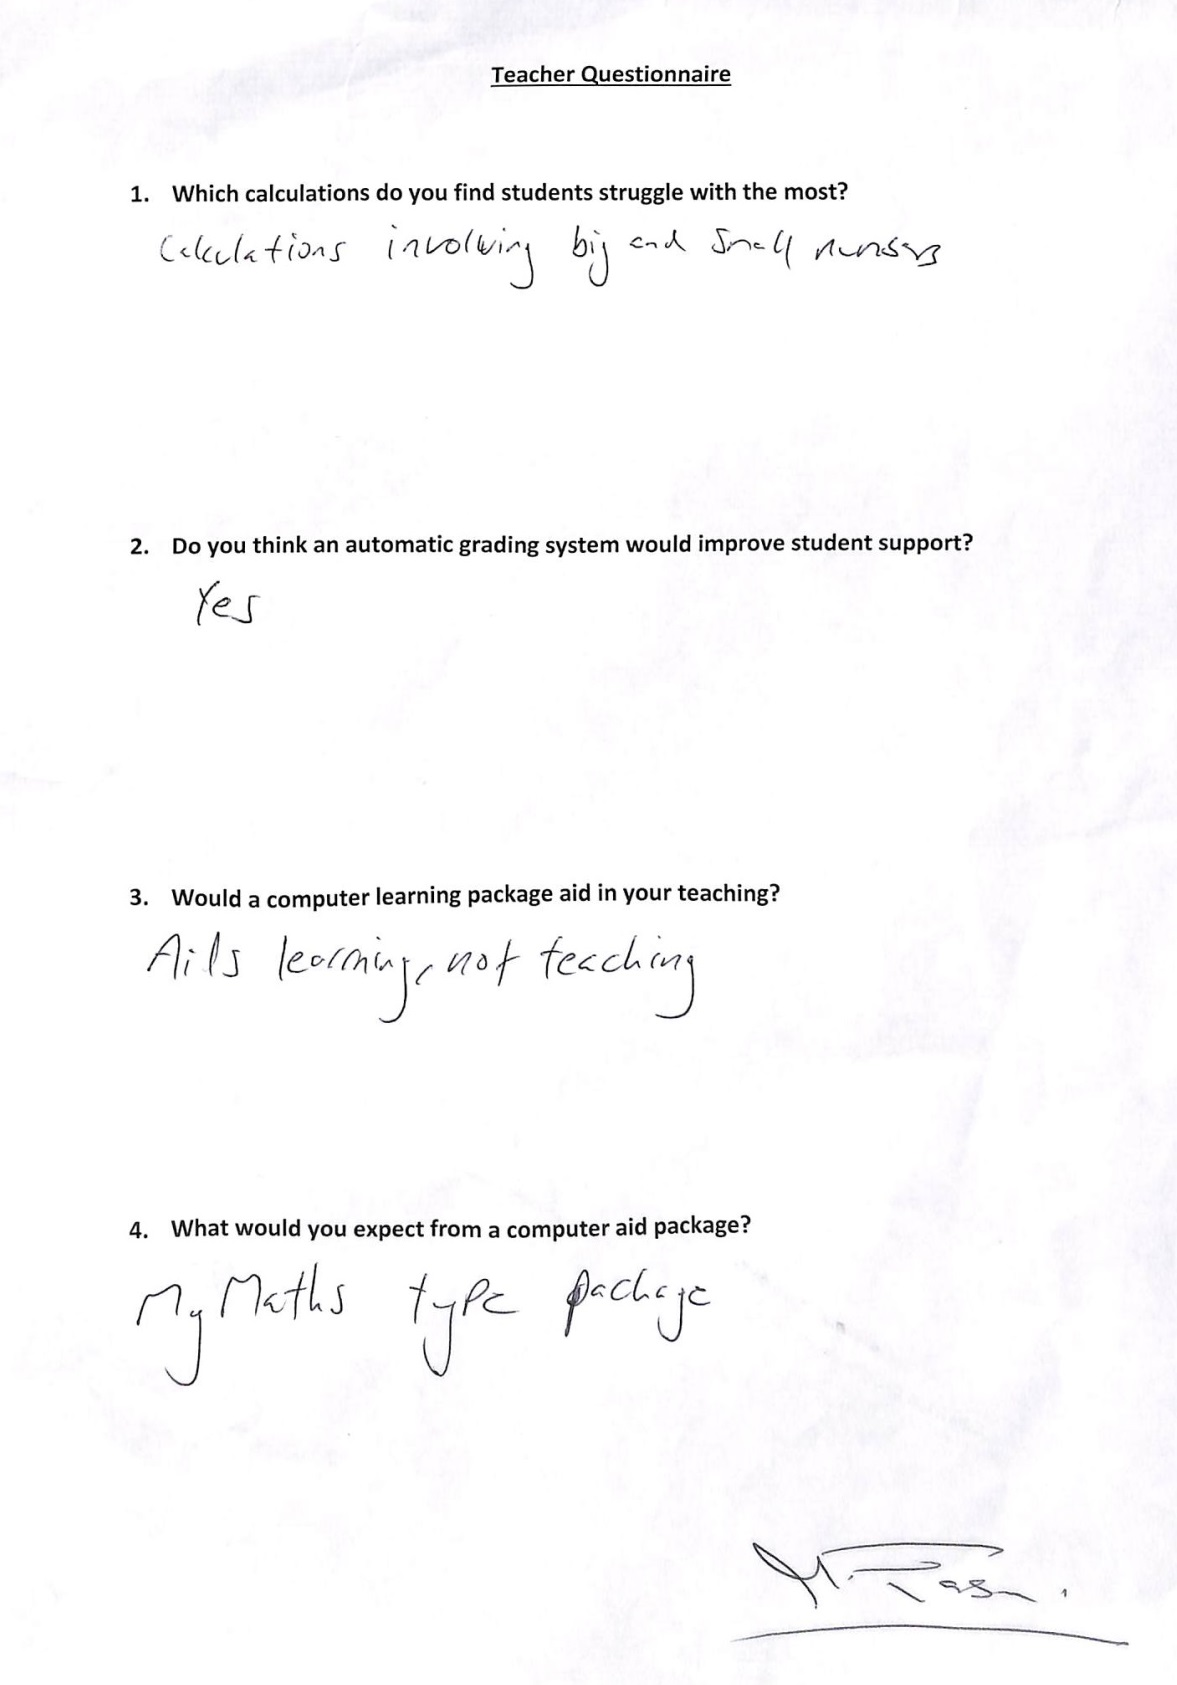
\includegraphics{TeacherQuestionnaire}

\clearpage
\section{Proposed System}        

Pupils will need to be able to input their own problems and have them be solved in a step by step process where they can enter their answer for each step. The program will tell them if they were right and instructing them as to what they should be doing. They will also be able to store their own problems and solutions in the central database.  Teachers will be allowed to set work to be done and see the scores. Teachers and pupils will also have unique accounts with teachers having the ability to see pupil scores and set questions. If pupils are having difficulties then they can send a message to the teacher and vice versa. Teachers should be able to make new pupil and teacher accounts and delete old ones.  Allows students and staff to log in. Won’t generate own questions as without use of libraries it would not be possible to display questions in the correct format. Only 100 questions will be stored at once as the memory taken up would be too high. Pupil accounts would have to be entered in manually as school will not give me access to the student detail database.\\

\section{Objectives}


\textbf{Essential Objectives}\\
\begin{enumerate}
\item Example Based Demonstration – The program should be able to provide a clear demonstration of how any of the equations work, by executing them for the user. It should be able to carry out this demonstration either on data entered by the user, or on data stored within the program/database.
\item Background Explanation Of Problems- The program should be able to give a small amount of detail initially if the student should request it
\item Interactive System allowing Users to Solve Equations – The user should be able to choose to attempt to solve the equations themselves – if this is the case the program should point out (or correct) any mistakes they may have made.
\item Unique User Accounts- Teachers and pupils should have different accounts with different privileges.
\item A System To Allow Users to Input and Store Questions – The users should be able to input their own questions, that the program can solve or walk them through, and have the option to store them.
\item A Database Holding Question Data- the program should run off of a back end database holding around 100 questions in total, which can randomly select a question, or allow a teacher to set specific questions for the pupil to answer.
\item A System For Teachers to set questions and Students Send Feedback – The program should allow teachers to select questions from the database to give to students. Students should be able to send feedback to their teachers.
\item A Database Holding Pupil Performance- Teachers should have access to the questions that pupils answered correctly and incorrectly so that they can monitor their performance and therefore provide support.
\end{enumerate}

\textbf{General Objectives}\\
\begin{enumerate}
\item Teachers should be able to create or delete user accounts.
\item  A central database should collate all information into a practical form.
\item The program should be self-explanatory and not overly complex for the user.
\item Should use less than 100MB of storage.
\item Grade scores. Highlights students who are below their target grades
\item Allows for students to make comments on problems so the teacher can help them.
\item A log in system with passwords and usernames
\end{enumerate}

\textbf{Acceptable Limitations}\\
\begin{enumerate}
\item  To allow the program to generate questions properly with the correct units would require the use of libraries and a lot more time than I have available.
\item  As my school will not allow me access to the student details database, students must be entered in manually.
\item  Only 100 questions stored at one time to control database size. As there may be hundreds of students inputting questions, the database may have thousands of questions at one time, which would make it cumbersome to use.
\item As the school already has a functioning email system, it would be unnecessary to recreate this system in my project.
\item  As having a function to solve equations could lead to cheating, I will leave this out.
\end{enumerate}

\chapter{Design}
\section{Navigation}

Log in menu
	Main Menu
		Set Questions *
			Select Student/s*
			Select Question/s*
		See Set Work 
			Attempt Set Questions
		Messages
			Open Messages
			Create Message
				Recipient
				Content
		Practice
			Finding K Questions
				Select question from list / Randomly
			Finding Rate Of Reaction Questions
				Select question from list / Randomly

\end{document}